% Scalar instruction entry source: tools/generate_scalar_instruction_catalog.py.
\subsection{\texttt{SETC.TGT}}
\label{sec:scalar-setc_tgt}
\index{SETC.TGT@\texttt{SETC.TGT}}
\begin{sloppypar}\noindent\textbf{Purpose.} Sets the block-commit condition/argument consumed by subsequent conditional block transitions.\end{sloppypar}\smallskip
\noindent\textbf{Syntax.}\par
\begin{lstlisting}[style=ptoscalarcode]
setc.tgt SrcL
\end{lstlisting}
\noindent\textbf{Encoding.}\par
\noindent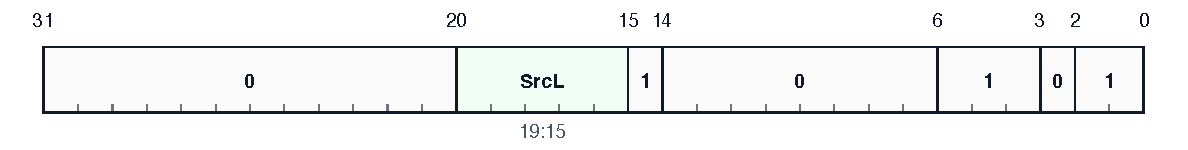
\includegraphics[width=\textwidth]{figs/encoding/scalar_instruction_entries/enc_setc_tgt.pdf}\par\smallskip
\begin{description}[leftmargin=0.18\linewidth,style=nextline]
\item[Format] \texttt{L32} \texttt{32-bit} scalar word.
\item[Pattern] \texttt{000000000000.....100000000111011}.
\end{description}
\noindent\textbf{Classification.}\par
\begin{description}[leftmargin=0.18\linewidth,style=nextline]
\item[Category] System, Cache, SSR, and Execution Control.
\item[Family] SSR Access.
\item[Execution class] \texttt{SYS}; uop\_kind=SYS, sys\_kind=SSR.
\end{description}
\noindent\textbf{Operand fields.}\par
\begin{description}[leftmargin=0.18\linewidth,style=nextline]
\item[\texttt{SrcL}] Bits \texttt{19:15 (5b)}. 5-bit scalar source register used as the left input operand.
\end{description}
\noindent\textbf{Operation.}\par
\begin{lstlisting}[style=ptoscalarcode]
SetCommitTarget(Read(SrcL))
\end{lstlisting}
\Needspace{0.08\textheight}
